% ---
\documentclass{article}


% Packages
% ---
\usepackage{amsmath,amssymb,amsthm} 	% Advanced math typesetting
% \usepackage[utf8]{inputenc} 	% Unicode support (Umlauts etc.)
\usepackage[USenglish]{babel} 	% Change hyphenation rules
\usepackage{hyperref} 				% Add a link to your document
\usepackage{graphicx}				% Add pictures to your document
\graphicspath{ {./images/} }	% image directory
\usepackage{listings} 				% Source code formatting and highlighting
\lstset{basicstyle=\ttfamily}		%Typewriter font for code writing
\usepackage{geometry}
\geometry{margin=1in}
\usepackage{enumitem}
\usepackage{float}
%\floatstyle{boxed}
\restylefloat{figure}
\usepackage{mathabx}
\usepackage{fancyhdr}
\usepackage[dvipsnames]{xcolor}
\usepackage[makeroom]{cancel}

\theoremstyle{definition}
\newtheorem{definition}{Def}

\pagestyle{fancy}
\fancyhf{}
\lhead{\bf CPSC 322 \\ Week 3 }
\rhead{\bf Jeremi Do Dinh \\ 61985628}
\rfoot{Page \thepage}



\usepackage{tikz}						% Graph drawing tools
\usetikzlibrary {positioning}

\usepackage{breqn}
\usepackage{multicol} 				% Multiple column functionality
\usepackage{blindtext}

\begin{document}

\noindent \url{https://www.cs.ubc.ca/~jordon/teaching/cpsc322/2019w2/}
\section*{Lecture VII}
\url{https://www.cs.ubc.ca/~jordon/teaching/cpsc322/2019w2/lectures/lecture7.pdf}

\subsection*{Heuristic Search}
Uninformed/blind algorithms don't take into account the goal node, until they actually are at the goal node. Often there is extra knowledge that can be used to guide the search: \textbf{{\color{blue} an estimate of the distance from node $ n $ to the goal node}}. This is called a \textbf{\textsl{{\color{blue} heuristic}}} \\ \\
\textbf{Definition (search heuristic):} 
A \textbf{{\color{blue} search heuristic $ h(n) $}} is an estimate of the cost of the lowest-cost path from node $ n $ to a goal node.
\begin{itemize}
	\item $ h $ can be extended to paths: $ h( \langle n_0, ..., n_k \rangle ) = h(n_k) $
	\item For now we think of $ h(n) $ as only using readily obtainable information about a node. 
\end{itemize}
\textbf{Definition (admissible heuristic):} A search heuristic $ h(n) $ is \textbf{{\color{blue} admissible}} if it is never an overestimate of the minimum cost from $ n $ to a goal.
\begin{itemize}
	\item There is never a path from $ n $ to the goal with path cost less than $ h(n) $
	\item \textit{Interpretation}: $ h(n) $ is a lower bound on the cost of getting from $ n $ to the nearest goal. 
\end{itemize}

\subsection*{How to construct an Admissible heuristic}
Identify a {\color{blue} \textit{relaxed} version of the problem}:
\begin{itemize}
	\item where one or more constraints have been dropped
	\item fewer restrictions on the actions
\end{itemize}
\textbf{Robot:} the agent {\color{blue} can move through walls}\\
\textbf{Driver:} the agent {\color{blue} can move straight to the destination}\\
\textbf{8-puzzle:} (1.) The tiles {\color{blue} can move anywhere} or (2.) tiles can move to {\color{blue} any adjacent square}. \\ \\
\textbf{\color{OliveGreen} Result:} The cost of an optimal solution in the relaxed problem is an admissible heuristic for the original problem. 
\subsubsection*{Example:}
\textbf{Search Problem}: robot has to find a route from start location to goal location on a grid (discrete space with obstacles). \\
\textbf{Final cost}: (quality of the solution) is the number of steps
 \begin{figure}[H]
	\centering
	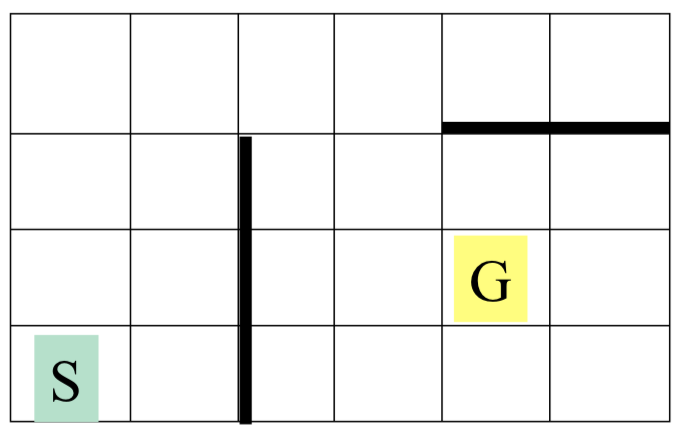
\includegraphics[width = 2.5in]{Pic2}
\end{figure}
\noindent If there are no obstacles, the cost of the optimal solution is (also referred to as the "\textbf{\textit{Manhattan Distance}}"):
\begin{figure}[H]
	\centering
	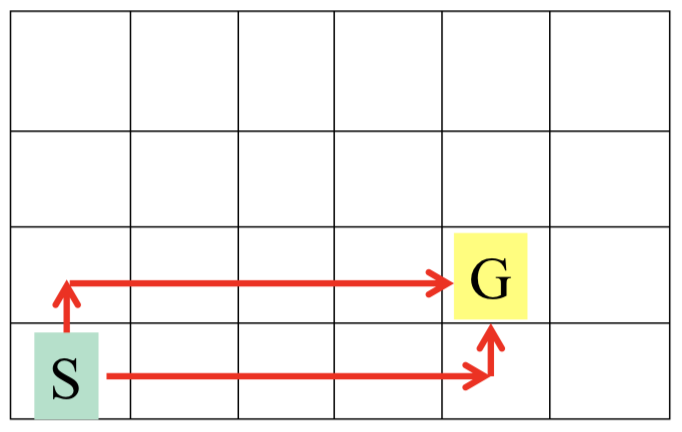
\includegraphics[width = 2.5in]{Pic3}
\end{figure}
\noindent If there are obstacles, then the \textbf{\color{blue} cost} of the optimal solution \textbf{\color{blue} without} obstacles is an \textit{\textbf{\color{blue} admissible heuristic}}. \\ \\
Similarly, consider the nodes being {\color{Magenta} points on a Euclidean plane} and the cost being the distance. Then we can use the linear distance from $ n $ to the nearest goal as the value of $ h(n) $. \\ \\
\textbf{\color{Dandelion} Clicker question}\\A reasonable admissible heuristic for the 8-puzzle is \textbf{\color{Dandelion} B}, the number of misplaced tiles: \\
Using the number of misplaced tiles is equivalent to assuming a tile can go anywhere, whether or not another tile is already at that location \\ \\
\textbf{In summary:} \\
We should identify constraints which, when dropped, make the problem extremely easy to solve
\begin{itemize}
	\item this is important because heuristics are not useful
if they're as hard to solve as the original problem!
\end{itemize}
\textbf{Another approach:} Solution cost of a sub-problem.

\subsection*{Heuristics: Dominance}
If $ h_1(n) \geq h_2(n) $ for every state $ n $ (both admissible), then $ h_2 $ \textbf{\color{blue} dominates} $ h_1 $. Then we know that $ h_2 $ is better for search! It provides a more accurate approximation. \\ \\
For the \textbf{8-puzzle problem}, we have the 2 heuristics:
\begin{enumerate}
	\item Tiles can move anywhere (number of misplaced tiles)
	\item Tiles can move to any adjacent square
\end{enumerate}
In this case we have that $ h_2(n) \geq h_1(n) $. 

\subsubsection*{How to combine heuristics when there is no dominance?}
\textbf{\color{Dandelion} Clicker question}\\ If $ h_1 $ and $ h_2 $ are both admissible, and dominance cannot be easily established, or is not consistent, then $ h(n) = \text{max}\{h_1, h_2\} $ (\textbf{\color{Dandelion} C}) is also admissible, \textbf{\color{blue} and dominates all its components}












\newpage
\section*{Lecture VIII}
\textbf{January 21st \& 23rd, 2020} \\
\url{https://www.cs.ubc.ca/~jordon/teaching/cpsc322/2019w2/lectures/lecture8.pdf}
 \subsection*{Admissible Heuristic for the Vacuum world}
 \begin{figure}[H]
 	\centering
 	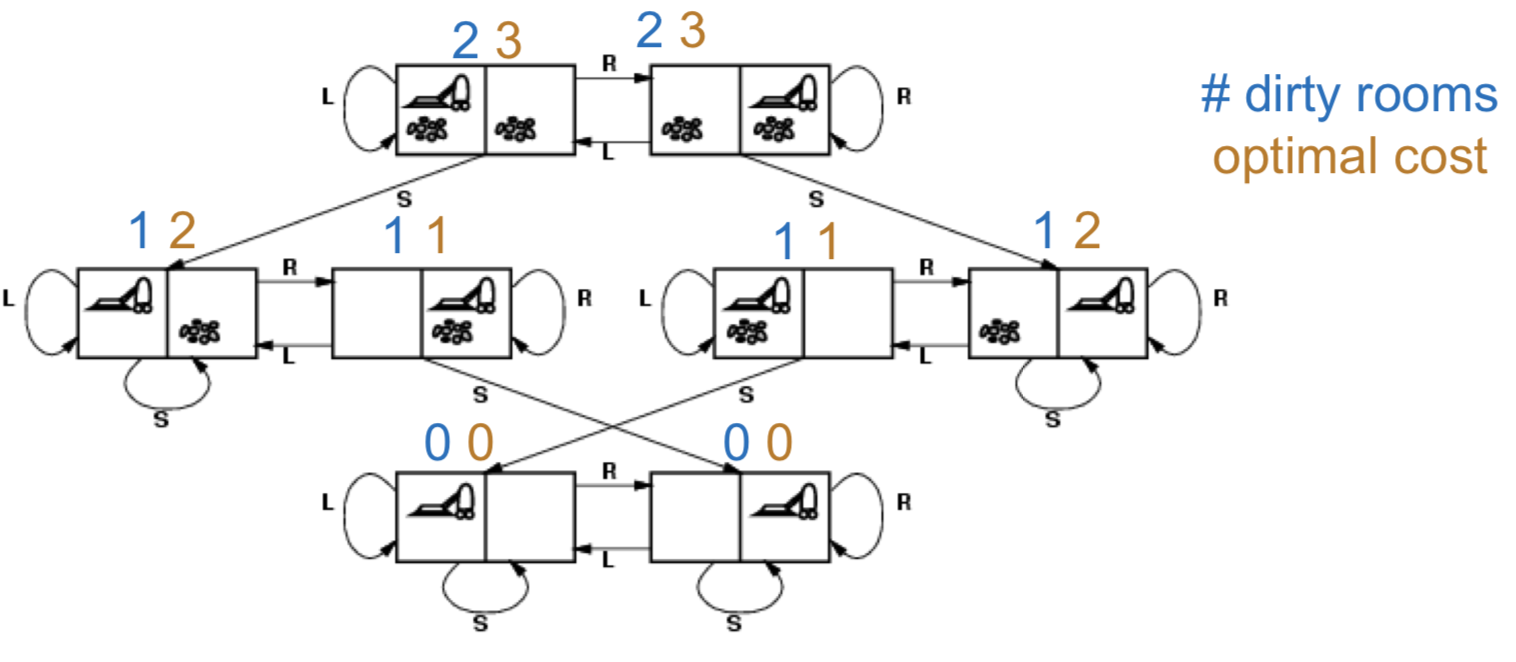
\includegraphics[width = 5in]{Pic1}
 	\caption{Heuristic in the vacuum world}
 \end{figure}
Above we have
\begin{itemize}
	\item States: \textit{Clean, Dirty, and robot location}
	\item Actions: \textit{Left, Right, Suck}
	\item Possible goal test: \textit{No dirt at all locations}
\end{itemize}

\subsection*{Best-First Search}
\begin{itemize}
	\item {\color{blue} \textbf{Idea:}} select the path whose end is closest to a goal according to heuristic function. 
	\item \textbf{Best-First Search} selects a path on the frontier with the minimal \textit{h}-value (for the end node).
	\item It treats the frontier {\color{blue} as a priority queue ordered by $ h $}
	\item This is a greedy approach, always chooses the path that looks locally best
\end{itemize}
\subsubsection*{Analysis of BFS}
\begin{itemize}
	\item {\color{blue} Not Complete}: low heuristic values in a cycle can mean that the cycle gets followed forever
	\item {\color{blue} Optimal}: No
	\item {\color{blue} Time complexity} is $ O(b^m) $
	\item {\color{blue} Space complexity} is $ O(b^m) $
\end{itemize}

\subsection*{A* search algorithm}
\textit{\textbf{A* is a mix of:}}
\begin{itemize}
	\item \textit{Lowest-cost-first search}
	\item \textit{Best-first search}
\end{itemize}
It treats the frontier as a priority queue ordered by {\color{OliveGreen} $ f(p) = \text{cost}(p) + h(p) $}. It always chooses the path on the frontier with the \textbf{lowest estimated total distance} from the goal.
\subsubsection*{Analysis of A*}
If the heuristic is completely uninformative (eg.: $ h = 0  $ everywhere), and all of the edge costs are the same, then \textbf{A*} is equivalent to BFS and LCFS. This is because when all costs ate the same LCFS is the same as BFS, and all the edges are the same beans that it is the same as \textit{BFS}.\\
For the remainder of the course we assume that all costs on the arcs are strictly positive. 

\subsubsection*{Optimality of A*}
\textbf{If A* return a solution, that solution is guaranteed to be optimal}, as long as:
\begin{itemize}
	\item The branching factor is finite
	\item the arc costs are strictly positive
	\item $ h(n) $ is an underestimate of the of the length of the shortest path from $ n $ to the goal node (i.e.: \textbf{\color{blue} Admissible}), and is non negative. 
\end{itemize} 
\textbf{Theorem:} If A* selects a path p as the solution, then p is an optimal (i.e., lowest-cost) path. \\ \\
\textbf{Proof:}
Consider the moment that \textbf{\textit{p}} is chosen from the frontier. Some part of path \textbf{\textit{p'}} will also be in the frontier. Let's call this path \textbf{\textit{p''}}. 
\begin{figure}[H]
	\centering
	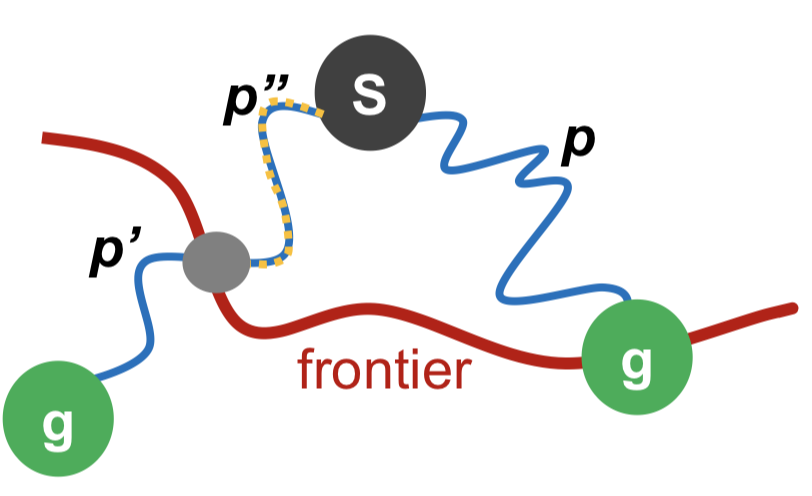
\includegraphics[width = 3in]{Pic4}
	\caption{Frontier at the moment that \textbf{\textit{p}} is chosen}
\end{figure}
Because \textbf{\textit{p}} was expanded before \textbf{\textit{p'}}, \textbf{\color{Plum} $ f(p) \leq h(p') $}. Therefore:
{\color{Plum}
\begin{align*}
\text{cost}(p) + h(p) \leq \text{cost}(p'') + h(p'')
\end{align*}}
But because \textbf{\textit{p}} ends at the goal, we have that {\color{Plum} $ h(p) = 0 $}. So:
{\color{Plum}
\begin{align*}
\text{cost}(p) + \cancel{h(p)} &\leq \text{cost}(p'') + h(p'')\\
\text{cost}(p) +  &\leq \text{cost}(p'') + h(p'')
\end{align*}}
Now, because $ h $ is admissible, we have that:
\begin{align*}
\text{cost}(p'') + h(p'') &\leq \text{cost}(p') 
\intertext{So combining both inequalities, we get:}
\text{cost}(p) &\leq \text{cost}(p')
\end{align*}
This \textit{contradicts} the assumption that $ p' $ is a better path. 
 \qed
\subsubsection*{Optimal efficiency of A*}
\begin{itemize}
	\item In fact, we can prove something even stronger about A*: in a sense (given the particular heuristic that is available) \textbf{\color{red} no search algorithm could do better!}
	\item \textbf{\color{blue} Optimal Efficiency}: Among \textbf{all optimal
		algorithms} that start from the same start node
		and \textbf{use the same heuristic} $ h $, \textsl{A*} {\color{blue} expands the
		minimal number of paths}.
\end{itemize}

\newpage

\section*{Lecture IX}
\textbf{January 23rd, 2020} \\
\url{https://www.cs.ubc.ca/~jordon/teaching/cpsc322/2019w2/lectures/lecture9.pdf}

\subsection*{Branch \& Bound search algorithm}
\begin{itemize}
	\item Follow exactly the same search path as DFS:
	\begin{itemize}
		\item \textbf{Treat the frontier as a stack}: expand the most recently added path first.
	\end{itemize}
\end{itemize}
\textbf{Idea:} Keep track of the {\color{blue} lower bound} and {\color{blue} upper bound} on solution cost at each path. 
\begin{itemize}
	\item {\color{blue} lower bound}: $ LB(p) = f(p) = \text{cost}(p) + h(p) $
	\item {\color{blue} upper bound}: $ UB =$ cost of the best solution found so far. We initialize $ UB = \infty $ (or some finite overestimate of the solution cost).
\end{itemize}
When a path $ p $ is selected for expansion:
\begin{itemize}
	\item If $ LB(p) \geq UB $, remove $ p $ from the frontier without expanding it (pruning).
	\item else, expand $ p $, adding all of its neighbors to the frontier.  
\end{itemize}

\subsubsection*{Branch-and-Bound Analysis}
\textbf{\color{Magenta} Completeness:} \textbf{not in general}, for the same reason that DFS isn't complete. 
\begin{itemize}
	\item however, for many problems of interest there are no infinite paths and no cycles
	\item also, you may be able to initialize the upper bound to some large finite number that is an overestimate of the solution cost
	\item hence, for many problems B\&B is complete
\end{itemize}
\textbf{\color{Magenta} Time-complexity:} $ O(b^m) $\\
\textbf{\color{Magenta} Space-complexity:} $ O(bm) $ (like DSF!). This is a big improvement over \textbf{A*} \\
\textbf{\color{Magenta} Optimality:} Yes, but not optimally efficient.

\subsection*{Pruning cycles, and Repeating cycles}

\subsubsection*{Cycle checking}
You can prune a path that ends in a node already on the path. This pruning cannot remove an optimal solution. In general the time complexity is \textbf{\color{blue} linear} in terms of path length.



\end{document}